\addcontentsline{toc}{chapter}{Appendix 3}
\chapter{State Transitions}

\begin{figure}[!htb]
\centering

\begin{tikzpicture}[->,>=stealth',shorten >=1pt,auto,node distance=8cm,semithick]
  \tikzstyle{every state}=[fill=red,draw=none,text=white]

  \node[initial,state] (A)                    {$A$};
  \node[state]         (B) [above right of=A] {$B$};
  \node[state]         (C) [below right of=B] {$C$};
  \node[state]         (D) [below right of=A] {$D$};

  \path (A) edge    [bend left]          node {$\alpha \wedge \beta$} (B)
        
        (B) edge [bend left]  node {} (A)
        
        (B) edge  [bend left] node {$\alpha \wedge \beta \wedge \gamma \wedge \delta$} (C)
        
        (B) edge [bend left] node [near end] {$\alpha \wedge \beta \wedge \gamma \wedge \delta \wedge \epsilon$} (D)
        
        (C) edge              node {} (A)
        (C) edge  [bend left] node [near start,above=10pt] {$\alpha \wedge \beta$} (B)
        
        
        (C) edge [bend left] node {$\alpha \wedge \beta \wedge \gamma \wedge \delta \wedge \epsilon$} (D)
        (D) edge [bend left]  node [near start] {$\alpha \wedge \beta$} (B)
        (D) edge [bend left] node {} (A);
        
\end{tikzpicture}
\caption{State transition diagram. The key to the symbols used for the transition conditions can be found in table \ref{tab:StateTransitionDiagramKey}.} \label{fig:StateTransitionDiagram}
\end{figure}

The Namuru Implementation use a number of different tracking loops depending on state. A state transition diagram can be seen in figure \ref{fig:StateTransitionDiagram}. In this diagram, 4 different states are visible. My thesis focuses on the carrier tracking loops, so a simplifying assumption is made that the receiver is always perfectly tracking the code phase. 

Given the robustness of the code phase tracking loops, this is a reasonable assumption.

In reality however, the receiver is initially in a acquisition state, where a delay doppler map is computed, in order to try and produce a rough estimate of the code and carrier phase.  An example of a delay doppler map can be seen in figures \ref{fig:DelayDopplerMap} and \ref{fig:DelayDopplerMapSubsection}.


\section{State A}
After acquisition, the receiver will achieve code lock almost immediately, at which point the receiver is in state A. Once the receiver is in state A, a FLL is initiated. The FLL is very simple in structure, consisting of a single proportional arm, with a gain of 0.125. As the receiver has not undergone bit alignment, the loop filter needs to be relatively insensitive to bit transitions. As alluded to before, a FLL with a finite gain is unable to completely remove the frequency error, however the goal of the pure FLL state is to get the receiver closer in frequency.

As alluded to before, the lock range of the receiver is given by:

\begin{equation}
\frac{-1}{2T} < f < \frac{1}{2T}
\end{equation}

When $T = 0.004$, the FLL has a locking range of $\pm 125Hz$. At the L1 frequency, 125Hz corresponds to $23.8ms^{-1}$. Accelerating at 15g ($147ms^{-2}$), the receiver needs to start locking within $\approx 160ms$, otherwise the doppler frequency will be outside the locking range.

\section{State B}
Once the receiver has been in the A state for at least 256ms, and once a filtered version of the frequency error is less then $30 \degree$, then the receiver transitions into state B.

State B uses a second order PLL with a first order FLL (Check this is correct). State B is also known as "Frequency lock".

\begin{comment}
The gain for the FLL can be computed from :  
$$T = (2\times0.001)$$
$$FLL1Bn = 5$$
$$FLL1C1 = \frac{T}{0.25}$$
$$K = FLL1B \times FLL1C1$$
$$K = 0.04$$
\end{comment}

The second order loop structure of the PLL can be seen in figure \ref{fig:SecondOrderLoopKaplan}. This 

\begin{figure}[!htb] 
    \centering
    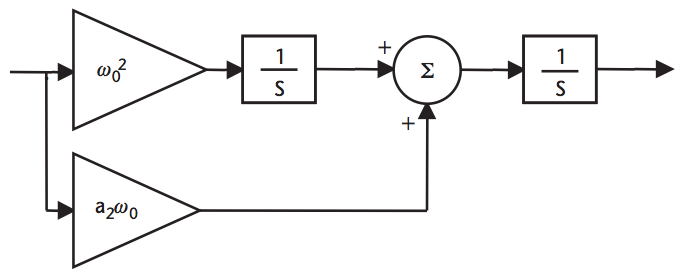
\includegraphics[width=1\textwidth]{Images/LoopArchitectures/SecondOrderLoop.png}
    \caption{Second order loop structure.}
    \label{fig:SecondOrderLoopKaplan}
\end{figure}


\section{State C}
Once the receiver has been in state B for at least 256ms, and if at least 20 of the past 32 measurements have a phase error of less than 30 degrees, then the receiver transitions to state C.

State C has exactly the same loop structure as state B, however the receiver is now considered to be in "phase lock", and data extraction can begin.

\section{State D}

Once the receiver has been in state C for at least 1280ms, the receiver transitions to state D. State D has a 3rd order PLL and a 2nd order FLL.



